

The various operations of the Fibonacci Heaps are as follows:
\begin{itemize}
	\item Inserting a node
	\item Union of Fibonacci Heaps
	\item Extracting the Minimum Node
	\item Decreasing a key
	\item Deleting a node
\end{itemize}

Let us consider $n$ to be the number of nodes in the Fibonacci Heap.

\subsection{Inserting a node}
In Fibonacci Heap, inserting a node is $O(1)$ operation since it is equivalent to adding a node to a circular, doubly linked list called the root list Figure~\ref{fig:Insertion1} and Figure~\ref{fig:Insertion2} . The added node has no children and is unmarked.
\begin{figure}[H]
	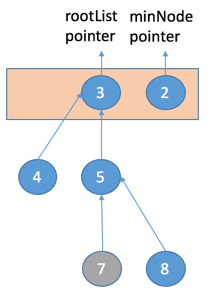
\includegraphics[scale=0.75]{Figures/FibonacciHeapBeforeInsertionOperation}
	\caption{Fibonacci Heap before Insertion}
	\label{fig:Insertion1}
\end{figure}
\begin{figure}[H]
	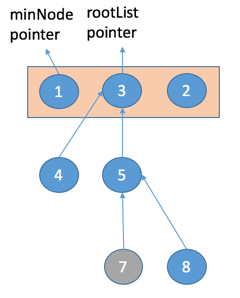
\includegraphics[scale=0.75]{Figures/FibonacciHeapAfterInsertionOperation}
	\caption{Fibonacci Heap post Insertion of a node of key 1}
	\label{fig:Insertion2}
\end{figure}
\subsection{Union of Fibonacci Heaps}
In Union operation, the root list of both the Fibonacci Heaps are united  and the new minimum node is determined Figure~\ref{fig:Union1} and Figure~\ref{fig:Union2}  . The amortized cost of the union operation is $O(1)$ as well.

\begin{figure}[H]
	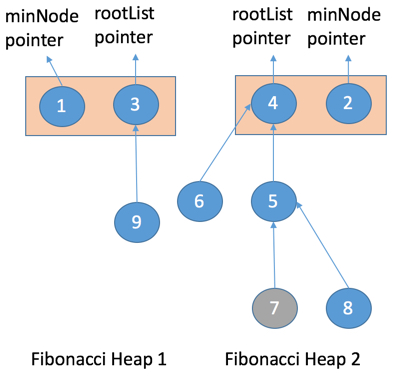
\includegraphics[width=0.95\columnwidth]{Figures/FibonacciHeapBeforeUnionOperation}
	\caption{Two Fibonacci Heap before Union Operation}
	\label{fig:Union1}
\end{figure}
\begin{figure}[H]
	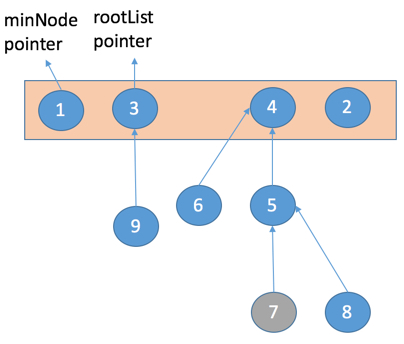
\includegraphics[width=0.95\columnwidth]{Figures/FibonacciHeapAfterUnionOperation}
	\caption{Fibonacci Heap after Union Operation}
	\label{fig:Union2}
\end{figure}



\subsection{Extracting the Minimum Node}
In the process of extracting the minimum node, the minimum node is extracted from the Fibonacci Heap. The procedure followed is as follows:
\begin{itemize}
	\item The minimum node's children are added to the root list.Figure~\ref{fig:extractMin1}
	\item Consolidate the root list by linking roots when they are of equal degree.Figure\ref{fig:extractMin2}
	\item Repeat the previous step until at most one root remains of each degree.Figure\ref{fig:extractMin3}
	\item Update the minimum node with the minimum key in the root list.Figure~\ref{fig:extractMin4}
\end{itemize}
The amortized cost of extracting a minimum node is $O(\lg{n})$

\begin{figure}[h]
	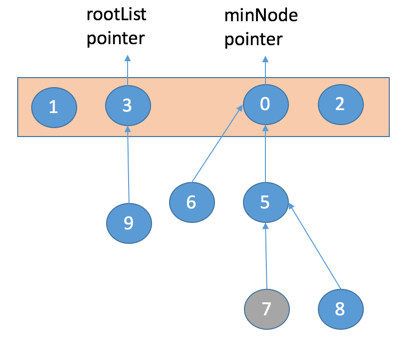
\includegraphics[width=0.95\columnwidth]{Figures/FibonacciHeapStep1ExtractMinOperation}
	\caption{The minimum node's children are added to the root list}
	\label {fig:extractMin1}
\end{figure}
\begin{figure}[h]
	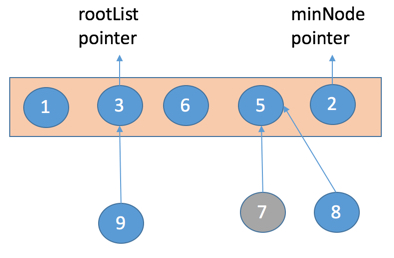
\includegraphics[width=0.95\columnwidth]{Figures/FibonacciHeapStep2ExtractMinOperation}
	\caption{Consolidate Operation}
	\label {fig:extractMin2}
\end{figure}
\begin{figure}[h]
	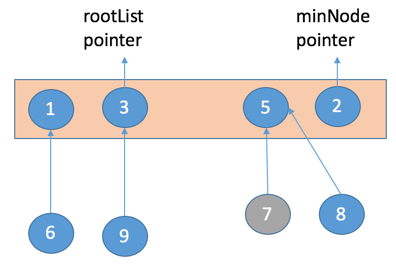
\includegraphics[width=0.95\columnwidth]{Figures/FibonacciHeapStep3ExtractMinOperation}
	\caption{Repeat the previous step until at most one root remains of each degree.}
	\label {fig:extractMin3}
\end{figure}
\begin{figure}[h]
	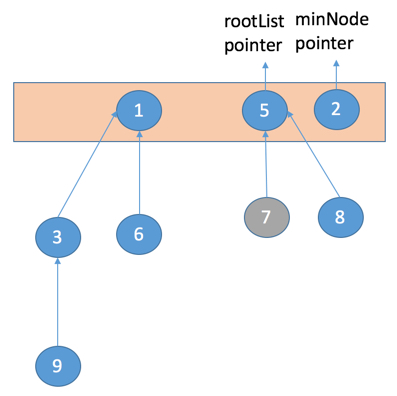
\includegraphics[width=0.95\columnwidth]{Figures/FibonacciHeapStep4ExtractMinOperation}
	\caption{Updating the Minimum Node pointer}
	\label {fig:extractMin4}
\end{figure}





\subsection{Decreasing a key}
In this process, we decrease the value of the key for an existing node. If the min-heap order is not violated, we need to update the minimum node if required Figure~\ref{fig:decreaseKey1NoViolation} and Figure~\ref{fig:decreaseKey2NoViolation} . If the min-heap order is violated, many changes can occur. The procedure followed is as follows:
\begin{itemize}
	\item We cut the node from it's parent Figure~\ref{fig:decreaseKey1Violation} and Figure~\ref{fig:decreaseKey2Violation} .
	\item Add the node to the root list Figure~\ref{fig:decreaseKey3Violation} . 
	\begin{itemize}
	\item If the parent is not marked, the parent is marked Figure~\ref{fig:decreaseKey3Violation}.
	\item If the parent was already marked, it would be added to the root list as well and this step occurs recursively up the tree until either a root or an unmarked node is found Figure~\ref{fig:decreaseKey3Violation} .
	\end{itemize}
	\item If the decreased key is less than the minimum node's key, we update the minimum node Figure~\ref{fig:decreaseKey4Violation} . 
\end{itemize}
The amortized cost of decreasing a key is $O(1)$


\begin{figure}[h]
	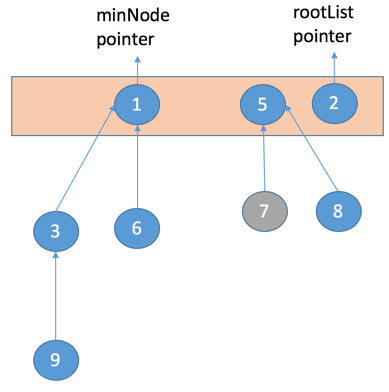
\includegraphics[width=0.95\columnwidth,height=0.75\columnwidth]{Figures/FibonacciHeapDecreaseKeyNoVilolation1Operation}
	\caption{Fibonacci Heap before decreasing the key 5 to 0}
	\label {fig:decreaseKey1NoViolation}
\end{figure}
\begin{figure}[h]
	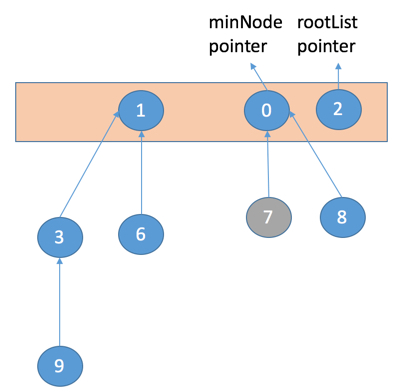
\includegraphics[width=0.95\columnwidth,height=0.75\columnwidth]{Figures/FibonacciHeapDecreaseKeyNoVilolation2Operation}
	\caption{Fibonacci Heap after decreasing the key 5 to 0}
	\label {fig:decreaseKey2NoViolation}
\end{figure}
\begin{figure}[h]
	\centering 
	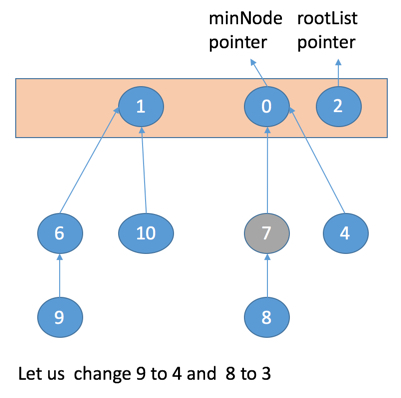
\includegraphics[width=0.95\columnwidth,height=0.75\columnwidth ]{Figures/FibonacciHeapDecreaseKeyVilolation1Operation}
	\caption{Fibonacci Heap before decreasing a key which violates the min-heap property}
	\label {fig:decreaseKey1Violation}
\end{figure}
\begin{figure}[h]
	\centering 
	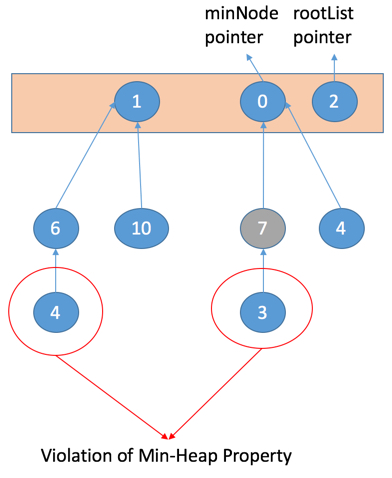
\includegraphics[width=0.95\columnwidth,height=0.75\columnwidth]{Figures/FibonacciHeapDecreaseKeyVilolation2Operation}
	\caption{Nodes with key 4 and 3 violate the min-heap property}
	\label {fig:decreaseKey2Violation}
\end{figure}
\begin{figure}[h]
	\centering 
	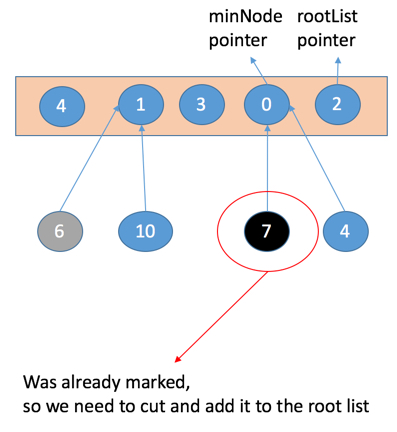
\includegraphics[width=0.95\columnwidth,height=0.75\columnwidth]{Figures/FibonacciHeapDecreaseKeyVilolation3Operation}
	\caption{Node 4 and 3 are added to the root list. Node 6 is marked but node 7 was already marked so we unmark it and add it to the root list}
	\label {fig:decreaseKey3Violation}
\end{figure}
\begin{figure}[h]
	\centering 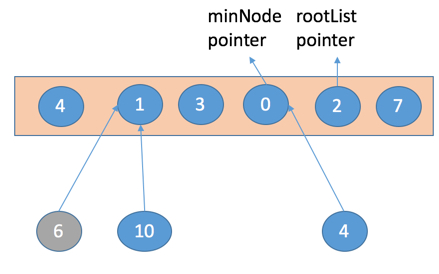
\includegraphics[width=0.95\columnwidth,height=0.75\columnwidth]{Figures/FibonacciHeapDecreaseKeyVilolation4Operation}
	\caption{Fibonacci Heap after decreasing the key 5 to 0}
	\label {fig:decreaseKey4Violation}
\end{figure}


\subsection{Deleting a node}
Deleting a node is equivalent to decreasing a key to -$ \infty $ and then extracting the minimum node (The node which whose key was updated to -$ \infty $ ) for a Fibonacci Heap and hence it has an amortized cost of $O(\lg{n})$ \\ \\ 